% ============================================================================
% Práctica: análisis del intercambio de mensajes V2X — Replay web 3D vs Wireshark
% Universidad de Cuenca — Redes Vehiculares y Heterogéneas (INGE-00104)
% Compilar: pdflatex -interaction=nonstopmode Practica_Replay_V2X.tex (x2)
% ============================================================================
\documentclass[11pt,a4paper]{article}

\usepackage[utf8]{inputenc}
\usepackage[T1]{fontenc}
\usepackage{lmodern}
\usepackage{amssymb}
\usepackage[margin=2.2cm]{geometry}
\usepackage{xcolor}
\usepackage{graphicx}
\usepackage{booktabs}
\usepackage{enumitem}
\usepackage{fancyhdr}
\usepackage{tikz}
\usetikzlibrary{positioning,arrows.meta}
\usepackage{listings}
\usepackage[most]{tcolorbox}
\usepackage{hyperref}

\definecolor{azul}{HTML}{002856}
\definecolor{rojo}{HTML}{A51008}
\definecolor{gris}{HTML}{58585B}
\definecolor{verde}{HTML}{1A7A4A}
\definecolor{fondocodigo}{HTML}{F5F5F5}

\hypersetup{colorlinks=true, linkcolor=azul, urlcolor=rojo, citecolor=azul}

\pagestyle{fancy}
\fancyhf{}
\fancyhead[L]{\small\color{azul}\textbf{Práctica · Mensajes V2X: web vs.\ Wireshark}}
\fancyhead[R]{\small\color{gris}Redes Vehiculares y Heterogéneas}
\fancyfoot[C]{\small\thepage}
\renewcommand{\headrulewidth}{0.6pt}

\lstdefinestyle{codigo}{
  backgroundcolor=\color{fondocodigo},
  basicstyle=\ttfamily\footnotesize,
  keywordstyle=\color{azul}\bfseries,
  commentstyle=\color{verde}\itshape,
  stringstyle=\color{rojo},
  numbers=none, breaklines=true, frame=single,
  rulecolor=\color{gris!40}, framesep=4pt,
  showstringspaces=false, tabsize=2, columns=fullflexible, keepspaces=true }
\lstset{style=codigo}

\newtcolorbox{enmac}[1][]{colback=azul!4, colframe=azul, fonttitle=\bfseries, breakable,
  title={EN EL MAC (PC local) #1}}
\newtcolorbox{encontenedor}[1][]{colback=rojo!4, colframe=rojo, fonttitle=\bfseries, breakable,
  title={DENTRO DEL CONTENEDOR \texttt{van3twin} #1}}
\newtcolorbox{ennavegador}[1][]{colback=verde!5, colframe=verde, fonttitle=\bfseries, breakable,
  title={EN EL NAVEGADOR #1}}
\newtcolorbox{notabox}[1][]{colback=gris!6, colframe=gris, fonttitle=\bfseries, breakable,
  title={Nota#1}}
\newtcolorbox{tareabox}{colback=azul!5, colframe=azul, fonttitle=\bfseries, breakable,
  title={TAREA}}

\setlength{\parskip}{4pt}
\setlength{\parindent}{0pt}
\renewcommand{\contentsname}{Contenido}

% ============================================================================
\begin{document}

\begin{center}
  {\color{azul}\LARGE\bfseries Análisis del intercambio de mensajes V2X}\\[4pt]
  {\color{gris}\large Replay 3D en el navegador frente a disección con Wireshark, sobre los mismos \texttt{.pcap}}\\[6pt]
  {\small Universidad de Cuenca --- Redes Vehiculares y Heterogéneas (INGE-00104)\\
  Prof.\ Pablo Barbecho --- 25 de agosto de 2026}
\end{center}

\vspace{2pt}\hrule\vspace{8pt}

\tableofcontents

% ============================================================================
\section{Objetivo}
% ============================================================================

Cada nodo ns-3 del ejemplo EVA de VaN3Twin graba un \texttt{.pcap} con
\emph{todo} lo que su interfaz 802.11p transmitió y recibió: mensajes ETSI
reales (CAM, CPM, DENM) en ASN.1 UPER sobre BTP/GeoNetworking. Esta práctica
analiza esa misma evidencia con dos herramientas complementarias:

\begin{enumerate}[leftmargin=1.6em, itemsep=2pt]
  \item El \textbf{replay 3D del visor SUMO-GEO}: reproduce la corrida sobre el
        mapa real, dibujando cada transmisión (pulso) y cada recepción (arco),
        con línea de tiempo, modo paso a paso y contenido decodificado al clic.
  \item \textbf{Wireshark}: disección protocolo a protocolo y campo a campo de
        cada trama, con filtros, gráficos de secuencia y estadísticas.
\end{enumerate}

Al terminar, el estudiante sabrá cuándo conviene cada vista y cómo se
complementan: \emph{dónde y cuándo} (web) frente a \emph{qué exactamente}
(Wireshark).

% ============================================================================
\section{Marco teórico}
% ============================================================================

\subsection{La pila ETSI ITS-G5}

Los mensajes de esta práctica viajan por la pila europea de ITS
(figura~\ref{fig:pila}). En la capa de \emph{acceso}, IEEE 802.11p (canal de
10\,MHz en 5,9\,GHz, modo OCB, sin asociación). Encima, la capa de
\emph{red y transporte}: \textbf{GeoNetworking} (EN 302 636-4-1, ethertype
\texttt{0x8947}) encamina por posición geográfica --- aquí en modo SHB
(\emph{Single Hop Broadcast}), cuyo encabezado incluye el \emph{Source
Position Vector} con posición, velocidad y rumbo del emisor --- y
\textbf{BTP} (EN 302 636-5-1), un transporte mínimo tipo UDP cuyo puerto
destino identifica el servicio: \texttt{2001} CAM, \texttt{2002} DENM,
\texttt{2009} CPM. Encima, la capa de \emph{facilities} genera los mensajes,
y sobre ella las aplicaciones (como la alerta de vehículo de emergencia del
EVA).

\begin{figure}[h!]
\centering
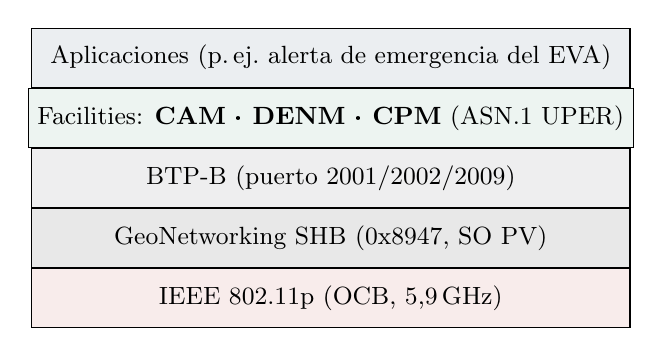
\begin{tikzpicture}[font=\small, node distance=0mm,
  capa/.style={draw, minimum width=76mm, minimum height=7.5mm, align=center}]
  \node[capa, fill=azul!8]  (app) {Aplicaciones (p.\,ej.\ alerta de emergencia del EVA)};
  \node[capa, fill=verde!8, below=of app] (fac) {Facilities: \textbf{CAM · DENM · CPM} (ASN.1 UPER)};
  \node[capa, fill=gris!10, below=of fac] (btp) {BTP-B (puerto 2001/2002/2009)};
  \node[capa, fill=gris!14, below=of btp] (gn)  {GeoNetworking SHB (0x8947, SO PV)};
  \node[capa, fill=rojo!8,  below=of gn]  (acc) {IEEE 802.11p (OCB, 5{,}9\,GHz)};
\end{tikzpicture}
\caption{Pila ITS-G5 tal como aparece en los \texttt{.pcap} de VaN3Twin.}
\label{fig:pila}
\end{figure}

\subsection{CAM --- Cooperative Awareness Message (EN 302 637-2)}

El ``latido'' de cada estación ITS: difunde periódicamente identidad y estado
cinemático para que los vecinos sepan que existe. Su frecuencia es
\textbf{adaptativa entre 1 y 10\,Hz}: se genera antes si la estación cambió
$\geq$4\,m de posición, $\geq$0,5\,m/s de velocidad o $\geq$4° de rumbo desde
el CAM anterior (y como máximo cada 1\,s). Estructura: \texttt{ItsPduHeader}
(protocolVersion, messageID$=$2, \textbf{stationID}) +
\texttt{generationDeltaTime} (ms mód.\ 65536) + contenedores:
\emph{basicContainer} (stationType, referencePosition),
\emph{highFrequencyContainer} (velocidad, rumbo, aceleración, curvatura,
dimensiones) y opcionalmente \emph{lowFrequencyContainer} (rol, luces,
trayectoria reciente).

\subsection{DENM --- Decentralized Environmental Notification (EN 302 637-3)}

Mensaje \textbf{por evento} (no periódico): notifica un peligro o situación
--- frenada brusca, obra, vehículo de emergencia en intervención --- con
\emph{causeCode}/\emph{subCauseCode}, posición del evento, área de relevancia
y validez temporal; se repite mientras el evento dura y puede cancelarse. En
el EVA, la ambulancia (stationType 10) dispara la lógica de alerta; los
receptores reaccionan (cambio de carril / ceder paso).

\subsection{CPM --- Collective Perception Message (TS 103 324)}

La ``percepción colectiva'': cada estación difunde lo que \emph{sus sensores}
ven --- objetos percibidos con posición, velocidad y dimensiones relativas ---
para que los demás ``vean a través'' de ella (peatones sin equipo V2X,
vehículos ocultos). Estructura: header (messageID$=$14) + contenedores de
gestión, información del emisor, de sensores y de \emph{objetos percibidos}.
En la corrida del EVA los verás como el tráfico más abundante junto a los CAM.

\subsection{ASN.1 y la codificación UPER}

Los tres mensajes se definen en \textbf{ASN.1} (Abstract Syntax Notation
One): un lenguaje de esquemas que separa el \emph{qué} (campos, rangos,
opcionalidad) del \emph{cómo se serializa}. ETSI publica los esquemas
(\texttt{.asn}) y VaN3Twin los incluye en
\texttt{src/automotive/model/ASN1/} --- son los mismos ficheros que el visor
usa para decodificar. En el aire se codifican con \textbf{UPER}
(\emph{Unaligned Packed Encoding Rules}): cada campo ocupa el mínimo de bits
que permite su rango, sin alineación a bytes --- por eso un CAM completo cabe
en $\sim$41 bytes. Consecuencias prácticas: los valores viajan como enteros
escalados que hay que interpretar con sus \textbf{unidades ETSI}
(tabla~\ref{tab:unidades}), y sin el esquema exacto la trama es ilegible ---
Wireshark y el visor decodifican porque conocen los \texttt{.asn}.

\begin{table}[h!]
\centering\small
\begin{tabular}{@{}llll@{}}
\toprule
\textbf{Campo} & \textbf{Unidad en el mensaje} & \textbf{Ejemplo} & \textbf{Valor real} \\
\midrule
latitude / longitude & $10^{-7}$ grados & 450523254 & 45,0523254° \\
speedValue & 0,01 m/s & 121 & 1,21 m/s \\
headingValue & 0,1° & 2700 & 270,0° \\
vehicleLengthValue & 0,1 m & 65 & 6,5 m \\
longitudinalAcceleration & 0,1 m/s$^2$ & 34 & 3,4 m/s$^2$ \\
generationDeltaTime & 1 ms (mód.\ 65536) & 523 & t $=$ \ldots{}523 ms \\
\bottomrule
\end{tabular}
\caption{Unidades ETSI de los campos que verás en el popup del visor y en Wireshark.}
\label{tab:unidades}
\end{table}

\subsection{Propagación radio: RSSI, dBm y el modelo log-distancia}
\label{sec:rssi}

\paragraph{Potencia en dBm.} El RSSI (\emph{Received Signal Strength
Indicator}) es la potencia de la señal recibida, expresada en dBm:
\[ P\,[\mathrm{dBm}] = 10\,\log_{10}\!\frac{P\,[\mathrm{mW}]}{1\,\mathrm{mW}}. \]
Es una escala logarítmica: $0$\,dBm $=1$\,mW, $+30$\,dBm $=1$\,W (la potencia
TX del EVA), $-45$\,dBm $=31{,}6$\,nW y $-85$\,dBm $=3{,}2$\,pW. Cada
$-10$\,dB es $10\times$ menos potencia; cada $-3$\,dB, la mitad.

\paragraph{Presupuesto de enlace.} La potencia que llega al receptor es
\[ \mathrm{RSSI} = P_{tx} + G_{tx} + G_{rx} - PL(d), \]
con $G$ las ganancias de antena (aquí $\approx 0$\,dBi) y $PL(d)$ la
\emph{pérdida de propagación} a distancia $d$. En espacio libre (Friis, con
$d$ en metros y $f$ en Hz):
\[ PL_{FS}(d) = 20\log_{10} d + 20\log_{10} f - 147{,}55 \;\mathrm{dB}
   \;\;\xrightarrow{f=5{,}9\,\mathrm{GHz}}\;\; 47{,}9 + 20\log_{10} d. \]

\paragraph{Modelo log-distancia.} El entorno real (edificios, suelo,
reflexiones) hace que la caída sea más rápida que en espacio libre. El modelo
estándar generaliza el exponente:
\[ PL(d) = PL(d_0) + 10\,n\,\log_{10}\!\frac{d}{d_0} \;(+\,X_\sigma), \]
donde $d_0$ es una distancia de referencia, $n$ el \textbf{exponente de
propagación} y $X_\sigma$ un término aleatorio de \emph{shadowing}
(sombras de obstáculos). Sustituyendo en el presupuesto de enlace, el RSSI
queda lineal en $\log_{10} d$:
\[ \boxed{\;\mathrm{RSSI}(d) = A - 10\,n\,\log_{10} d\;}
   \qquad A = \mathrm{RSSI}(1\,\mathrm{m}). \]

\begin{center}
\small
\begin{tabular}{@{}ll@{}}
\toprule
\textbf{Entorno} & \textbf{Exponente $n$ típico} \\
\midrule
Espacio libre & 2{,}0 \\
Urbano abierto (V2V con línea de vista) & 2{,}5--3{,}0 \\
Urbano denso / sin línea de vista & 3{,}0--4{,}5 \\
Interior con obstáculos & 4--6 \\
\bottomrule
\end{tabular}
\end{center}

\paragraph{Estimar $n$ a partir de dos medidas.} De la ecuación anterior:
\[ n = \frac{\mathrm{RSSI}(d_1)-\mathrm{RSSI}(d_2)}
            {10\,\log_{10}(d_2/d_1)}. \]
\emph{Ejemplo con datos reales de esta práctica} (etiquetas del visor):
$(6\,\mathrm{m}, -45{,}8\,\mathrm{dBm})$ y
$(135\,\mathrm{m}, -81{,}7\,\mathrm{dBm})$:
\[ n = \frac{-45{,}8-(-81{,}7)}{10\,\log_{10}(135/6)}
     = \frac{35{,}9}{13{,}5} \approx 2{,}66. \]
Regla práctica con $n\approx2{,}7$: \textbf{duplicar la distancia cuesta}
$10n\log_{10}2 \approx 8$\,\textbf{dB}.

\paragraph{Sensibilidad y alcance máximo.} El receptor decodifica mientras
$\mathrm{RSSI} \geq S$, donde $S$ es la \emph{sensibilidad} de esa tasa. La
tabla~\ref{tab:sens} recoge las ocho tasas del canal de 10\,MHz de 802.11p
con su modulación, el SNR aproximado que requieren y la sensibilidad
\textbf{mínima que exige la norma} (IEEE 802.11, con PER $\leq 10\,\%$ y
tramas de 1000 bytes); los receptores reales --- y los modelos de error de
ns-3 --- suelen ser 5--10\,dB mejores que ese mínimo.

\begin{table}[h!]
\centering\small
\begin{tabular}{@{}llll@{}}
\toprule
\textbf{Tasa (10 MHz)} & \textbf{Modulación} & \textbf{SNR req.\ aprox.} & \textbf{Sensib.\ mín.\ IEEE} \\
\midrule
3\,Mbit/s  & BPSK 1/2   & $\sim$5\,dB  & $-85$\,dBm \\
4,5\,Mbit/s& BPSK 3/4   & $\sim$6\,dB  & $-84$\,dBm \\
6\,Mbit/s  & QPSK 1/2   & $\sim$8\,dB  & $-82$\,dBm \\
9\,Mbit/s  & QPSK 3/4   & $\sim$9{,}5\,dB & $-80$\,dBm \\
\textbf{12\,Mbit/s} & \textbf{16-QAM 1/2} & $\sim$11\,dB & $-77$\,dBm \\
18\,Mbit/s & 16-QAM 3/4 & $\sim$14\,dB & $-73$\,dBm \\
24\,Mbit/s & 64-QAM 2/3 & $\sim$18\,dB & $-69$\,dBm \\
27\,Mbit/s & 64-QAM 3/4 & $\sim$19\,dB & $-68$\,dBm \\
\bottomrule
\end{tabular}
\caption{Tasas de 802.11p (canal de 10\,MHz). En negrita, la usada por el
EVA. A más orden de modulación, más bit/s pero más SNR requerido y peor
sensibilidad $\Rightarrow$ menos alcance.}
\label{tab:sens}
\end{table}

Despejando la distancia máxima desde una medida de referencia:
\[ d_{max} = d_{ref}\cdot 10^{\frac{\mathrm{RSSI}(d_{ref})-S}{10\,n}}. \]
Con la medida de 6\,m y una sensibilidad efectiva $S=-92$\,dBm (receptor
mejor que el mínimo normativo, como el modelo de ns-3):
$d_{max} = 6 \cdot 10^{(\!-45{,}8+92)/26{,}6} \approx 330$\,m --- coherente
con el ``rango máximo observado'' de $\sim$311\,m del panel PHY. Con el
mínimo IEEE ($-77$\,dBm) saldrían solo $\sim$90\,m: la diferencia ilustra
cuánto importa la calidad del receptor.

\paragraph{Modelos de canal en VaN3Twin.} La tabla~\ref{tab:modelos} resume
qué modelo de propagación usa cada tecnología en los ejemplos
\texttt{automotive} (verificado en el código del árbol):

\begin{table}[h!]
\centering\small
\begin{tabular}{@{}p{0.20\textwidth}p{0.72\textwidth}@{}}
\toprule
\textbf{Tecnología} & \textbf{Modelo de canal} \\
\midrule
802.11p (EVA y \texttt{v2v/v2i-*-80211p}) & \texttt{LogDistancePropagationLossModel} con $n=3{,}0$, referencia 46,7\,dB a 1\,m + \texttt{ConstantSpeed} (retardo). \textbf{Determinista}: sin shadowing ni fading. Alternativa lista (comentada en el EVA): \texttt{CniUrbanmicrocellPropagationLossModel} (WINNER+ B1, LOS/NLOS). \\
LTE / C-V2X Modo 4 & \texttt{cv2x\_CniUrbanmicrocellPropagationLossModel} (urbano microcelda). \\
NR-V2X & Canal 3GPP completo (TR 37.885/38.901), escenario \texttt{V2V\_Highway}: pathloss por escenario + shadowing configurable + LOS/NLOS dinámico + fast fading espacial. \\
Sionna (\texttt{*-sionna-*}) & Ray tracing NVIDIA sobre escena 3D (servidor externo). \\
\bottomrule
\end{tabular}
\caption{Modelos de propagación por tecnología en los ejemplos automotive.}
\label{tab:modelos}
\end{table}

Nota para el ejercicio de estimación: el $n\approx2{,}7$ ajustado con las
etiquetas del visor sale algo menor que el $n=3{,}0$ configurado porque el
punto más cercano (6\,m) pesa la zona de la distancia de referencia; con
puntos $\geq$40\,m el ajuste converge a $\sim$3.

\paragraph{SNR y ruido.} El margen de decodificación es
$\mathrm{SNR} = \mathrm{RSSI} - N$, con el suelo de ruido
\[ N = -174 + 10\log_{10}(BW) + NF
     \;\xrightarrow{BW=10\,\mathrm{MHz},\,NF\approx7\,\mathrm{dB}}\;
     \approx -97\,\mathrm{dBm}. \]
La tasa del EVA (16-QAM~1/2) requiere $\mathrm{SNR}\gtrsim 11$\,dB
(tabla~\ref{tab:sens}), de donde $S \approx -97+11 = -86$\,dBm: RSSI, SNR y
sensibilidad son caras de la misma moneda.

% ============================================================================
\section{Requisitos previos}
% ============================================================================

\begin{itemize}[leftmargin=1.6em, itemsep=2pt]
  \item Stack unificado van3twin + visor operativo
        (ver \texttt{Manual\_Simulacion\_VaN3Twin\_SUMO\_GEO.pdf}).
  \item Wireshark en el Mac: \texttt{brew install -{}-cask wireshark}.
  \item Una corrida del EVA ejecutada (Modo A o B; los \texttt{.pcap} se
        generan siempre).
\end{itemize}

% ============================================================================
\section{Parte 1 --- Generar la corrida y publicar los pcaps}
% ============================================================================

\begin{encontenedor}
\begin{lstlisting}[language=bash]
pkill -f ns3-dev-v2v; pkill sumo; sleep 1
./ns3 run "v2v-emergencyVehicleAlert-80211p --sumo-gui=false --met-sup=true --sumo-updates=0.1"
# al terminar, publicar las capturas y (opcional) limpiar las del arbol:
cp ~/VaN3Twin/ns-3-dev/v2v-EVA-*.pcap ~/results/
\end{lstlisting}
\end{encontenedor}

\begin{notabox}
Un fichero por nodo: \texttt{v2v-EVA-\emph{n}-0.pcap} es lo que \emph{vio} la
interfaz del nodo $n$ (sus TX propios y los RX que le llegaron). El pool de
nodos se reutiliza: si un vehículo sale de SUMO y entra otro, ambos comparten
pcap en tramos de tiempo distintos --- el replay web lo resuelve solo; en
Wireshark se distingue por el \texttt{stationID} del mensaje.
\end{notabox}

\begin{enmac}
\begin{lstlisting}[language=bash]
cd ~/van3twin-docker
# el backend detecta los ficheros nuevos automaticamente al pulsar Replay
curl localhost:8000/api/replay/info              # totales por tipo y PDR por par
\end{lstlisting}
\end{enmac}

\subsection*{Opcional: potencia de recepción real (RSSI/SNR) por mensaje}

Los pcap de ns-3 no llevan radiotap, pero VaN3Twin expone el RSSI/SNR de cada
mensaje recibido mediante \emph{SignalInfo} (parche del framework). Basta
volcarlo a un CSV que el replay ingiere automáticamente. En
\texttt{src/automotive/model/Applications/emergencyVehicleAlert.cc} (editar
dentro del contenedor, ver manual):

\begin{lstlisting}[language=C++, caption={1) \#include <fstream> junto a los dem\'as includes, y esta funci\'on ANTES de StartApplication (dentro del namespace ns3) --- en C++ debe estar definida antes de usarse}]
static void logSignalCSV (long tx, long rx, double rssi, double snr)
{
  static std::ofstream f ("signal-rx.csv", std::ios::trunc);
  static bool hdr = false;
  if (!hdr) { f << "rx,tx,t_ms,rssi,snr\n"; hdr = true; }
  f << rx << "," << tx << "," << Simulator::Now ().GetMilliSeconds ()
    << "," << rssi << "," << snr << "\n";
}
\end{lstlisting}

\begin{lstlisting}[language=C++, caption={2) En StartApplication, junto al addCARxCallback existente (l\'inea $\sim$261). Ambos callbacks conviven: el normal mantiene la l\'ogica del EVA. OJO: el campo es stationId (d min\'uscula) en los headers ASN.1 de este \'arbol.}]
  m_caService.addCARxCallbackExtended (
      [this] (asn1cpp::Seq<CAM> cam, Address from, StationId_t sid,
              StationType_t stype, SignalInfo phy)
      {
        logSignalCSV (asn1cpp::getField (cam->header.stationId, long),
                      std::stol (m_id.substr (3)), phy.rssi, phy.snr);
      });
\end{lstlisting}

\begin{lstlisting}[language=C++, caption={3) \'Idem para los CPM --- firma propia (Seq<CollectivePerceptionMessage> y StationID\_t), no reutilizar la lambda del CAM}]
  m_cpService.addCPRxCallbackExtended (
      [this] (asn1cpp::Seq<CollectivePerceptionMessage> cpm, Address from,
              StationID_t sid, StationType_t stype, SignalInfo phy)
      {
        logSignalCSV (asn1cpp::getField (cpm->header.stationId, long),
                      std::stol (m_id.substr (3)), phy.rssi, phy.snr);
      });
\end{lstlisting}
Tras \texttt{./ns3 build} y una corrida:
\texttt{cp signal-rx.csv v2v-EVA-*.pcap \textasciitilde/results/} --- el
backend detecta los ficheros nuevos automáticamente. El visor mostrará entonces \textbf{RSSI en las etiquetas de los
enlaces}, en los receptores del popup y como estadística en el panel PHY.
Formato aceptado del CSV (cabecera, orden libre):
\texttt{rx,tx,t\_ms,rssi[,snr]} --- stationID numéricos, tiempo en ms de
simulación, RSSI en dBm.

% ============================================================================
\section{Parte 2 --- Replay 3D en el navegador}
% ============================================================================

Abrir \url{http://localhost:8081}. La figura~\ref{fig:visor} muestra el
entorno completo en modo replay: paneles SUMO·GEO, Replay V2X y PHY 802.11p a
la izquierda, Históricos a la derecha, y sobre el mapa los pulsos de
transmisión de la flota.

\begin{figure}[h!]
\centering
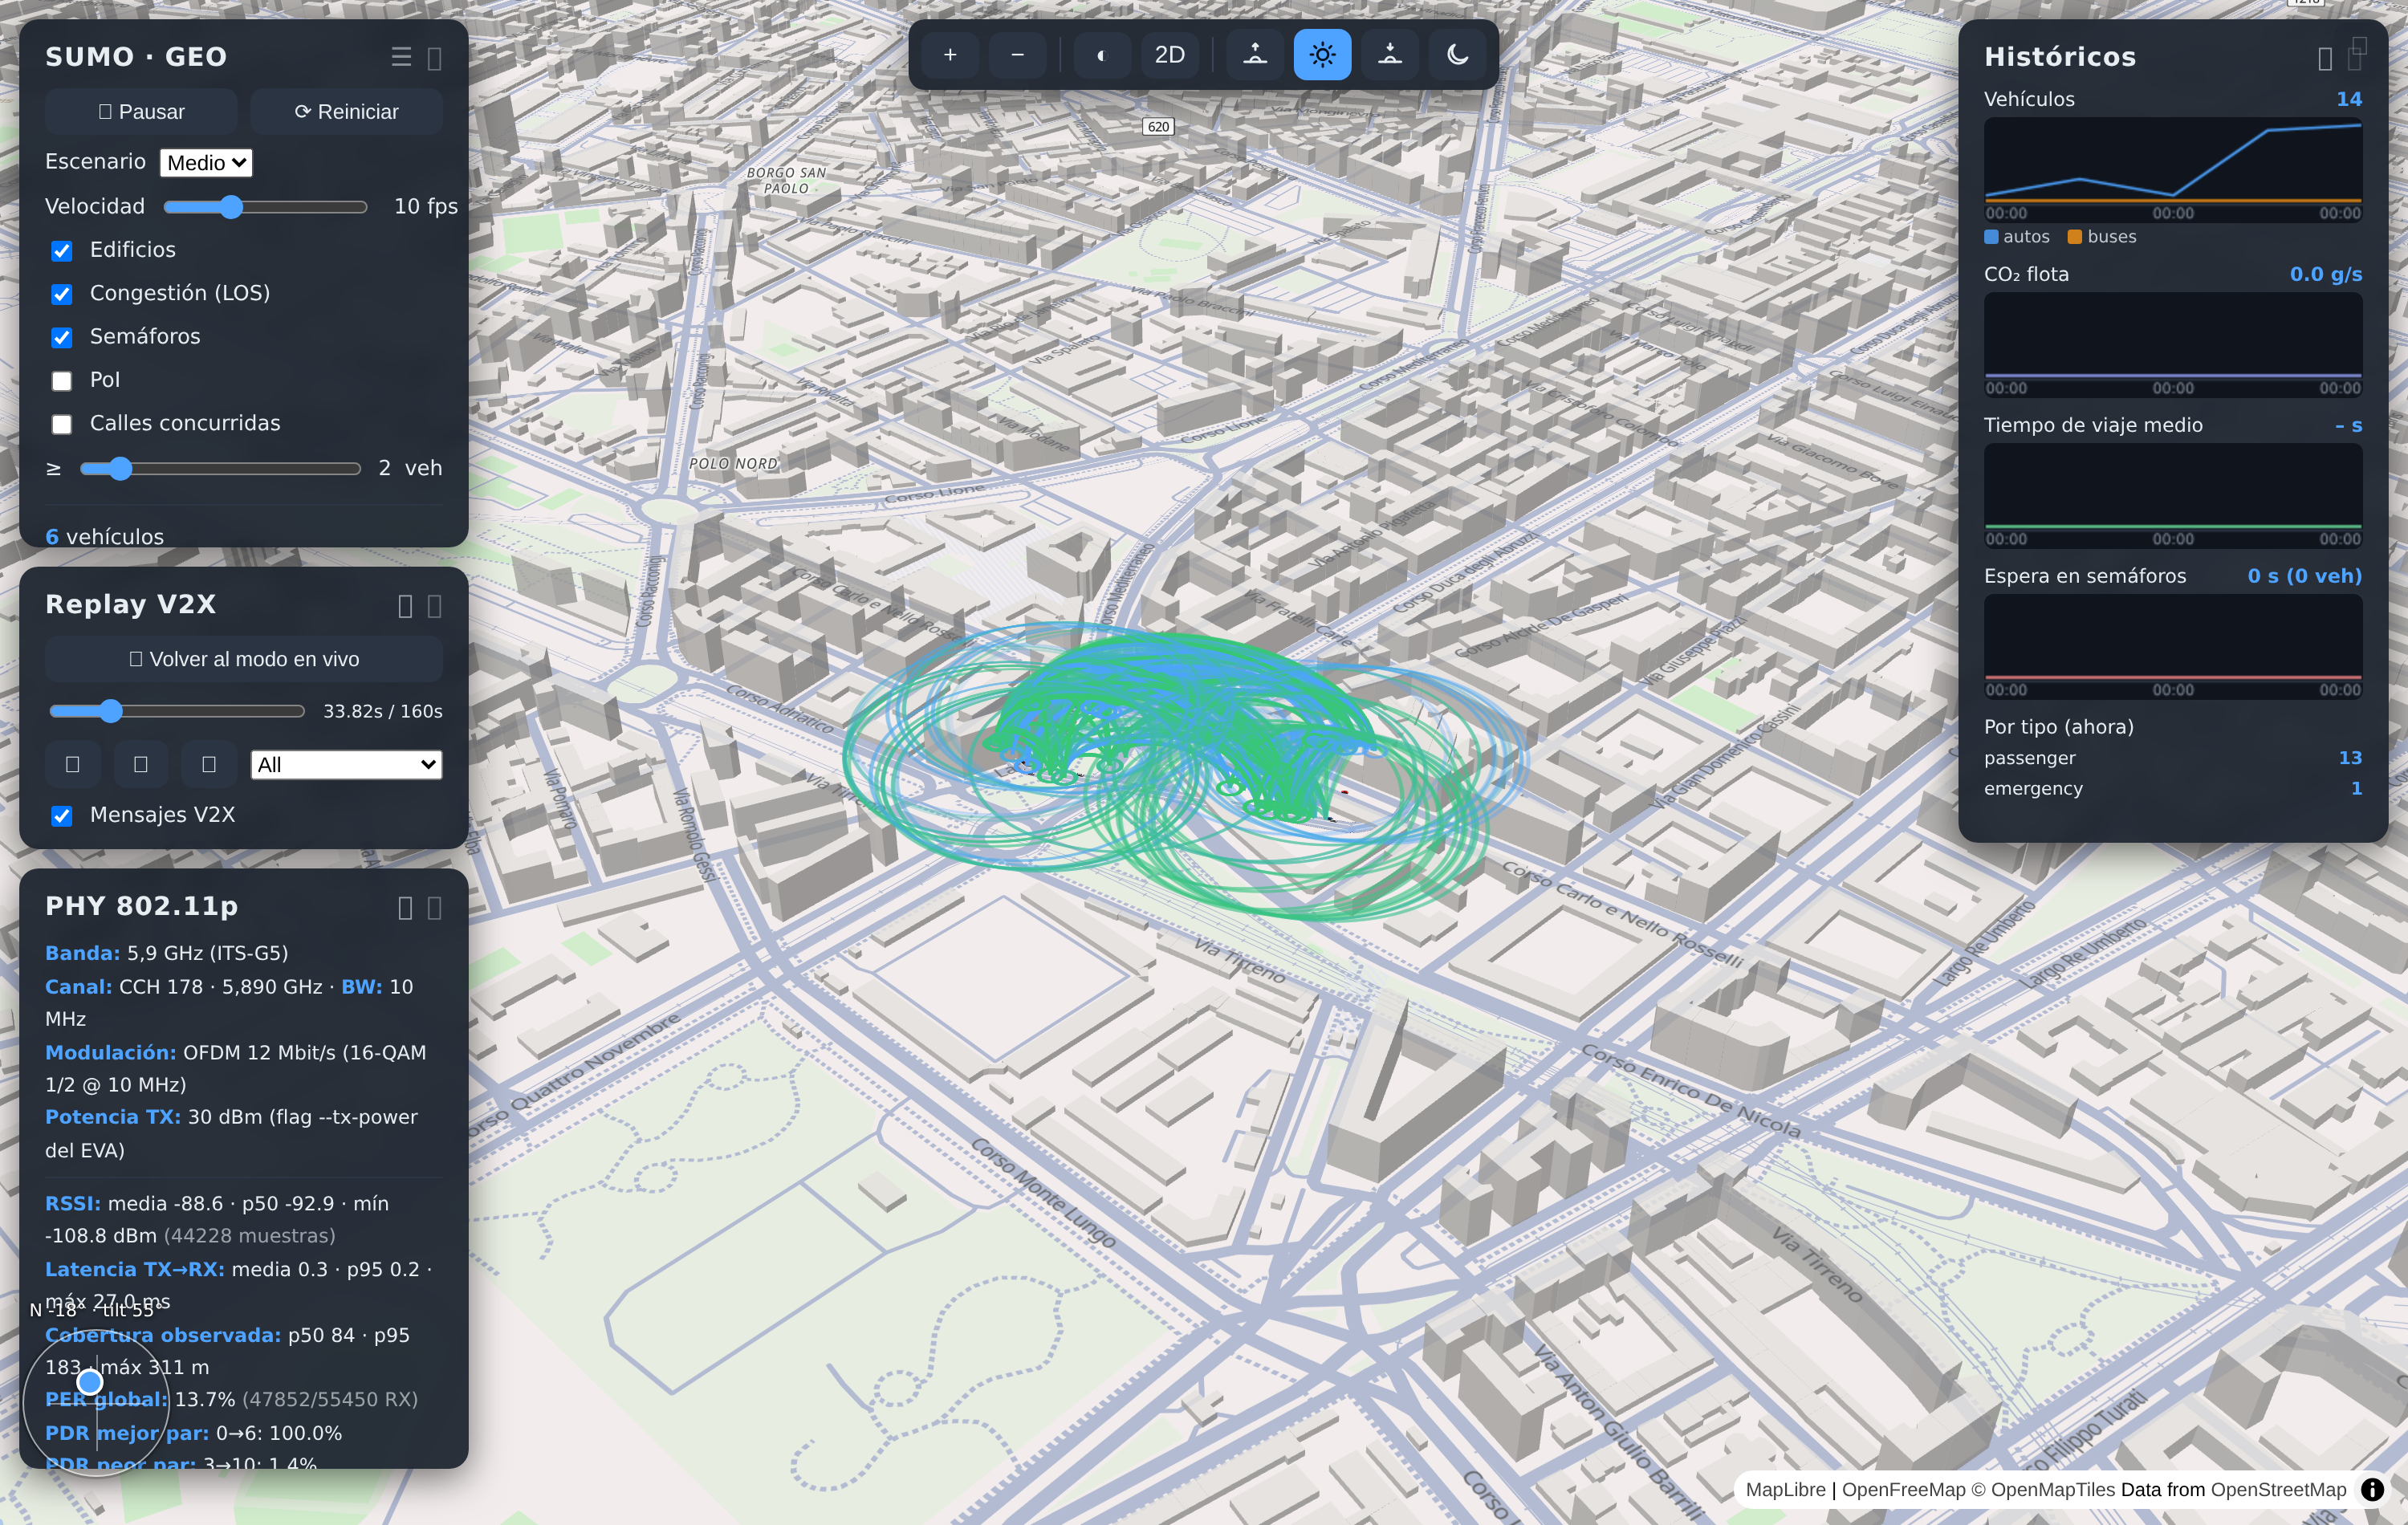
\includegraphics[width=\textwidth]{img/visor_general.png}
\caption{El visor en modo replay: cada círculo expandiéndose sobre el mapa es
una transmisión (CAM azul, CPM verde); los paneles muestran los controles y
las métricas PHY reales de la corrida.}
\label{fig:visor}
\end{figure}

Bajo el panel SUMO·GEO está el panel \textbf{Replay V2X} con todos los
controles (figura~\ref{fig:paneles}):

\begin{center}
\small
\begin{tabular}{@{}p{0.30\textwidth}p{0.62\textwidth}@{}}
\toprule
\textbf{Control} & \textbf{Función} \\
\midrule
\texttt{Replay pcap} & Conecta el visor a la corrida grabada (y de vuelta al modo en vivo) \\
Línea de tiempo & Posición actual; arrastrar $=$ \emph{seek} a cualquier instante \\
Botón $\blacksquare$/$\blacktriangleright$ (play/pausa) & Reproducir o pausar el replay desde el propio panel \\
Botones $\blacktriangleleft$ / $\blacktriangleright$ & Paso atrás / adelante: salta un frame (\texttt{APP\_STEP\_LENGTH}\,s) y pausa; los mensajes del paso quedan \textbf{congelados} en pantalla \\
Selector All/veh$X$ & Filtra pulsos y arcos a los \emph{emitidos} por ese vehículo, y lo resalta con un anillo ámbar en el mapa \\
CAM / CPM / DENM & Filtros por tipo (azul / verde / rojo) \\
Mensajes V2X & Muestra u oculta la capa completa \\
Panel \textbf{PHY 802.11p} & Métricas de capa física de la corrida: banda/canal/BW/modulación, potencia TX, latencia TX$\rightarrow$RX (media/p95/máx), rango de cobertura observado, PER global, PDR mejor/peor par, tasas y utilización de canal \\
\bottomrule
\end{tabular}
\end{center}

\begin{figure}[h!]
\centering
\begin{minipage}[t]{0.40\textwidth}
  \centering
  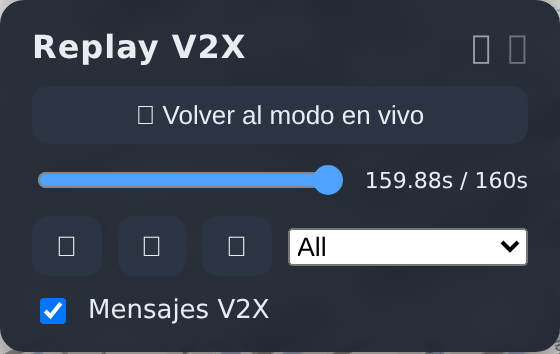
\includegraphics[width=\linewidth]{img/panel_replay.png}\\[4pt]
  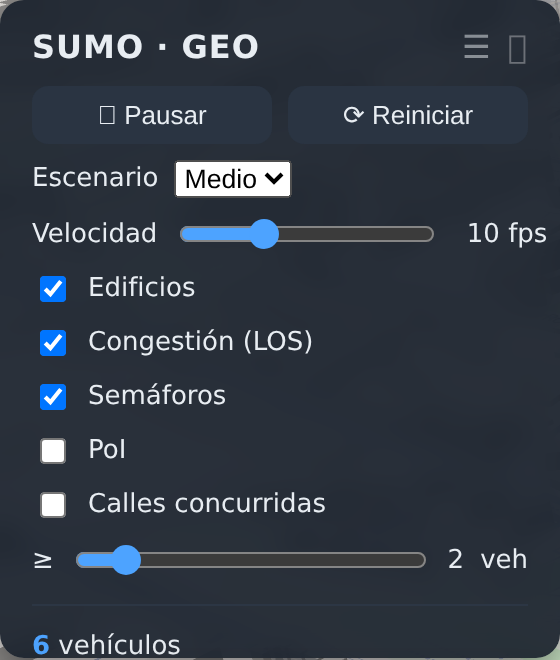
\includegraphics[width=\linewidth]{img/panel_sumogeo.png}
\end{minipage}\hfill
\begin{minipage}[t]{0.46\textwidth}
  \centering
  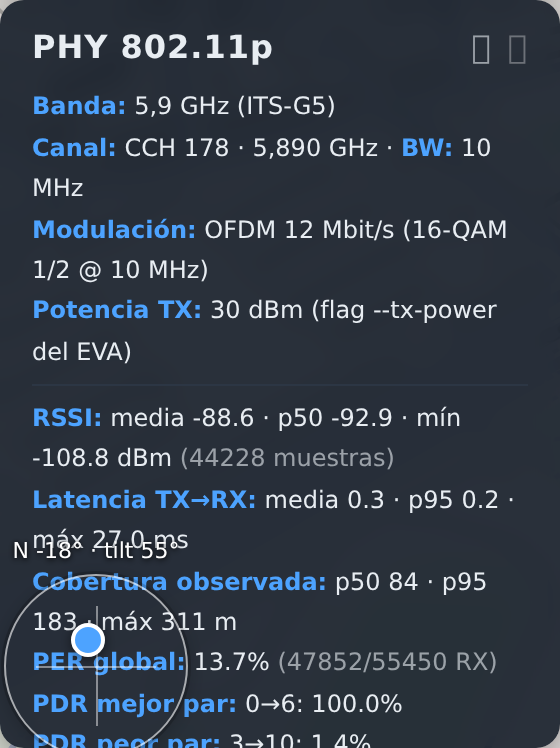
\includegraphics[width=\linewidth]{img/panel_phy.png}
\end{minipage}
\caption{Izquierda: panel Replay V2X (timeline, play/pausa, pasos
$\blacktriangleleft/\blacktriangleright$, selector de emisor y filtros) y
panel SUMO·GEO. Derecha: panel PHY 802.11p con las métricas medidas de la
corrida (RSSI, latencia, cobertura, PER, PDR, tasas).}
\label{fig:paneles}
\end{figure}

\begin{notabox}
La potencia RX por trama \textbf{no} está disponible en los pcap (sin
radiotap); con \texttt{signal-rx.csv} presente, el panel PHY añade la fila
RSSI (como en la figura~\ref{fig:paneles}). La latencia y el rango se
\emph{miden} emparejando cada recepción con su transmisión y las
trayectorias; el PER compara recepciones logradas con las esperadas según qué
vehículos coexistían.
\end{notabox}

\begin{ennavegador}[--- flujo sugerido]
1) \texttt{Replay pcap} $\rightarrow$ play: visión general (densidad de
pulsos $=$ carga de canal). 2) Elegir ``veh0'' (la ambulancia).
3) Paso a paso con $\blacktriangleright$ (y $\blacktriangleleft$ para
retroceder): en cada paso, observar qué arcos salen de veh0 y \textbf{clic
sobre el pulso o el arco} $\rightarrow$ \textbf{disección por capas
plegables}, como en Wireshark (IEEE 802.11 $\rightarrow$ GeoNetworking SHB
$\rightarrow$ BTP-B $\rightarrow$ ITS con el ASN.1 completo), más la lista de
receptores; el popup admite scroll y se cierra con la \texttt{X}. 4) \emph{Seek} al
tramo donde la ambulancia cruza el centro y comparar receptores cerca/lejos.
Interpreta los valores con la tabla~\ref{tab:unidades}. Las
figuras~\ref{fig:paso} y~\ref{fig:popup} muestran el resultado esperado.
\end{ennavegador}

\begin{figure}[h!]
\centering
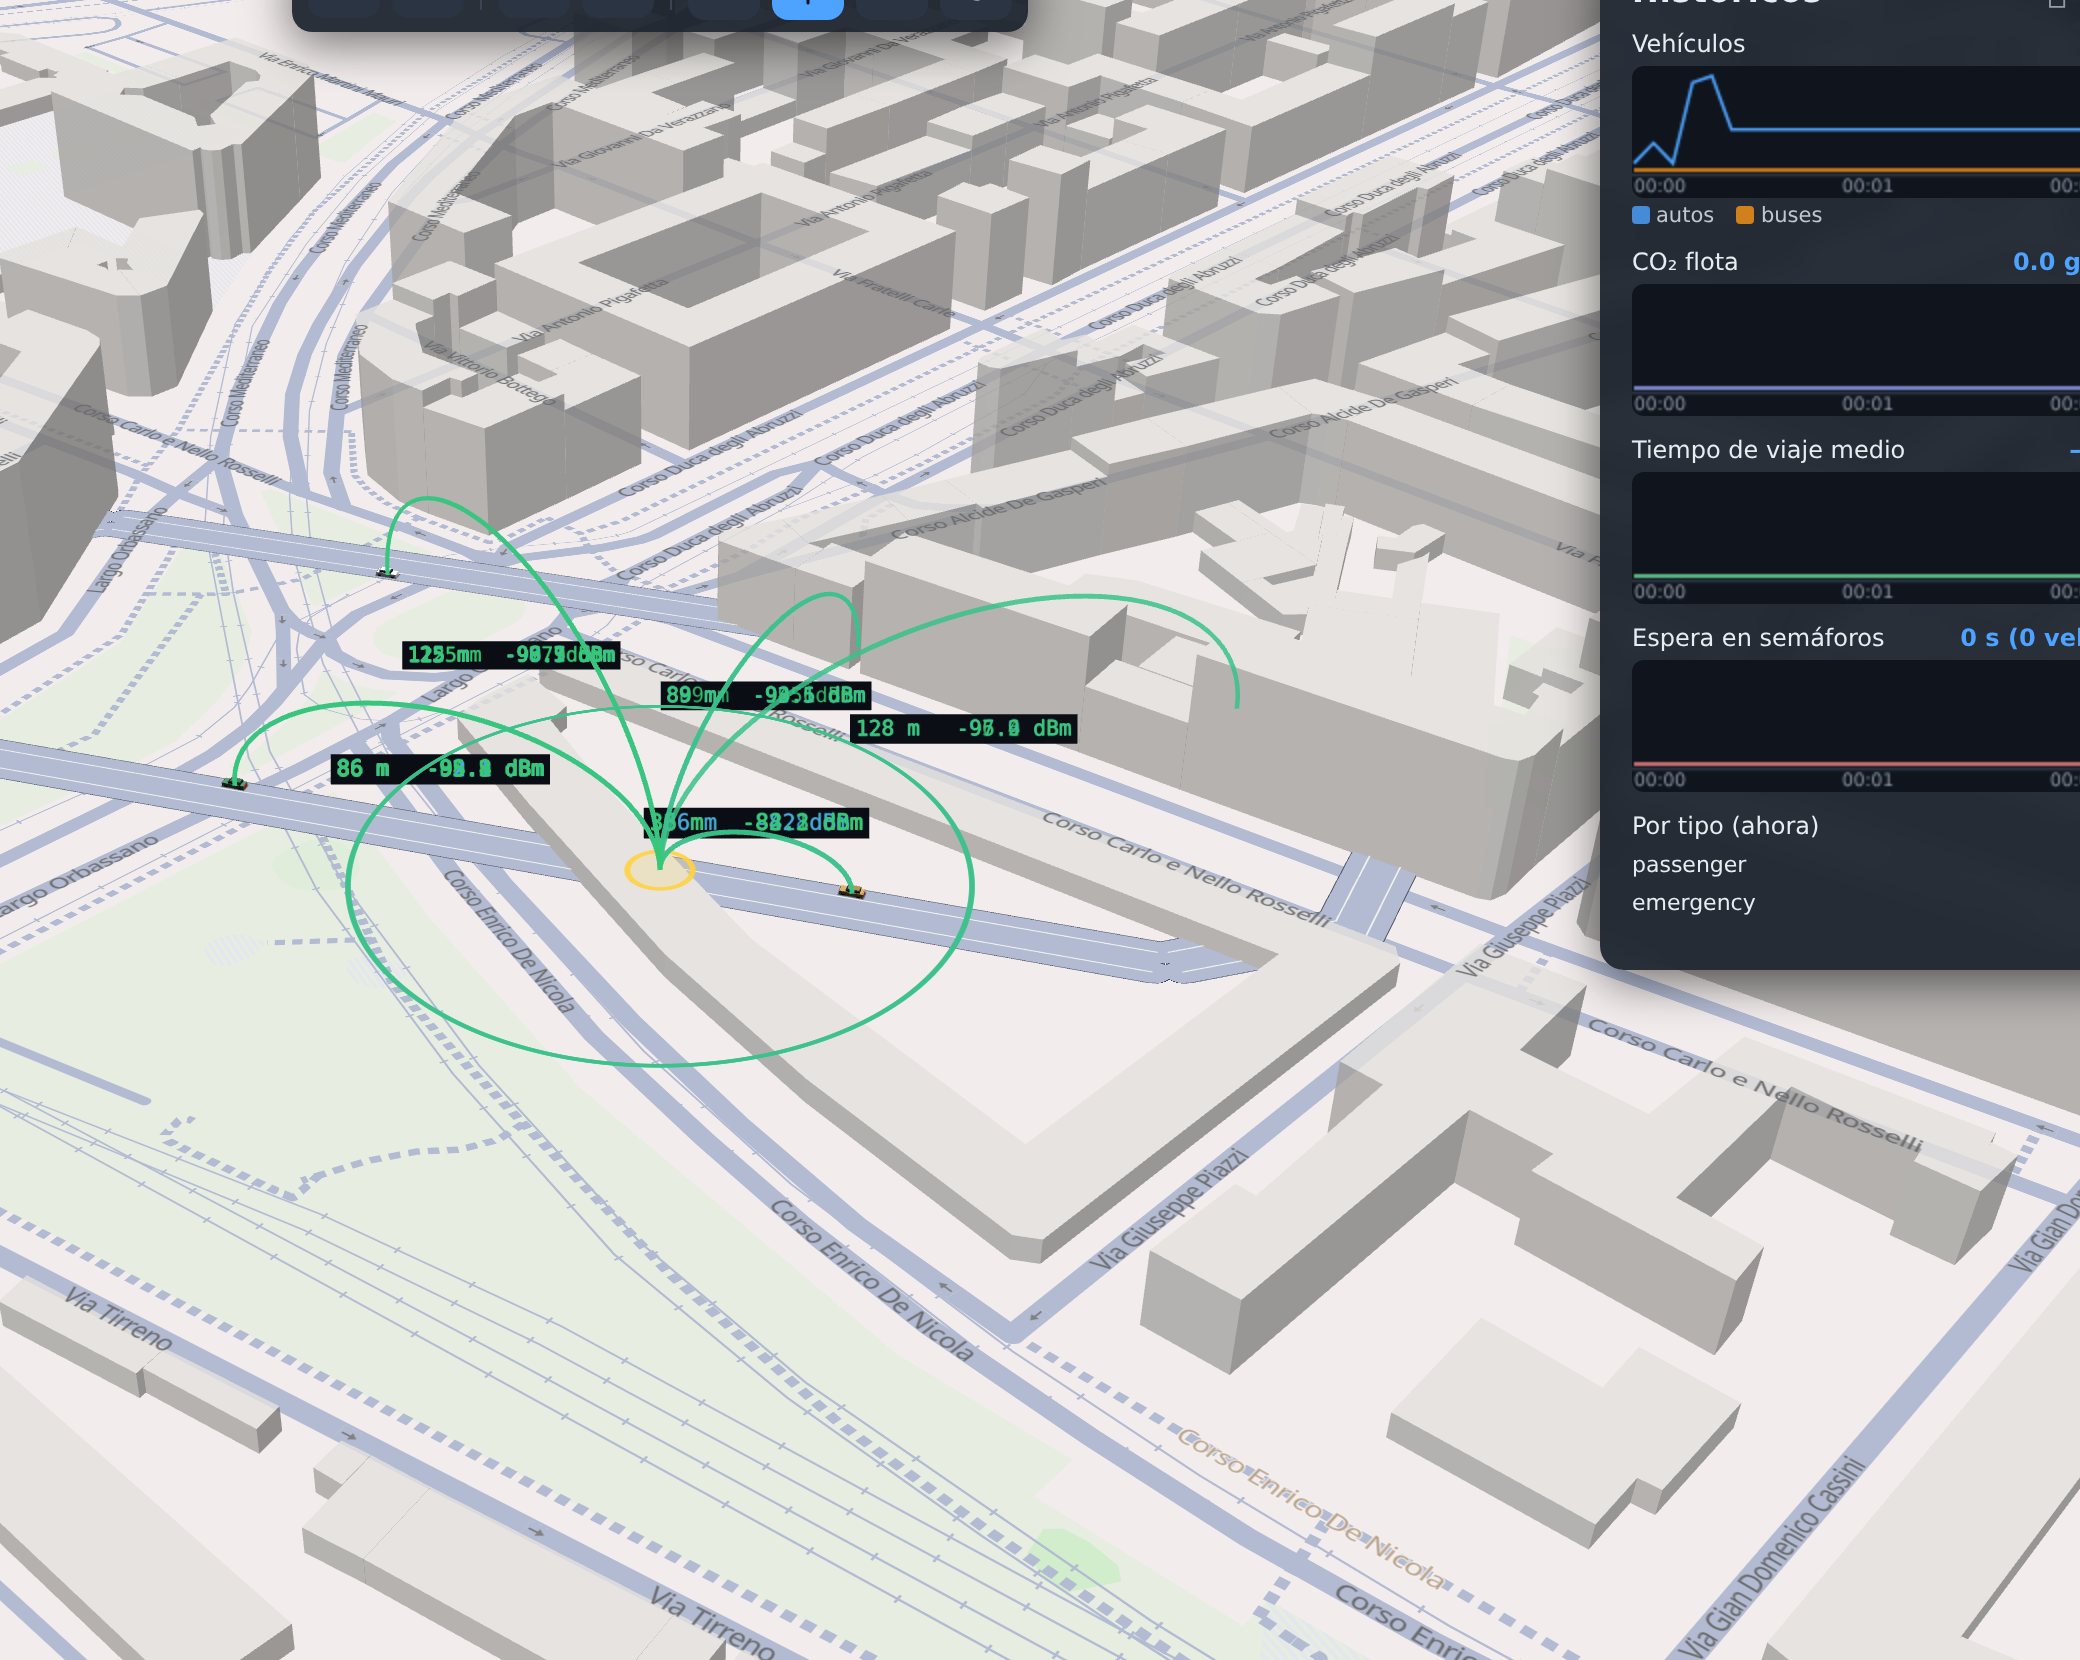
\includegraphics[width=0.92\textwidth]{img/replay_paso.png}
\caption{Modo paso a paso con la ambulancia (veh0) seleccionada: anillo ámbar
en el emisor, arcos verdes (CPM) hacia cada receptor con su etiqueta
\emph{distancia · RSSI}. Los mensajes quedan congelados para inspeccionarlos.}
\label{fig:paso}
\end{figure}

\begin{figure}[h!]
\centering
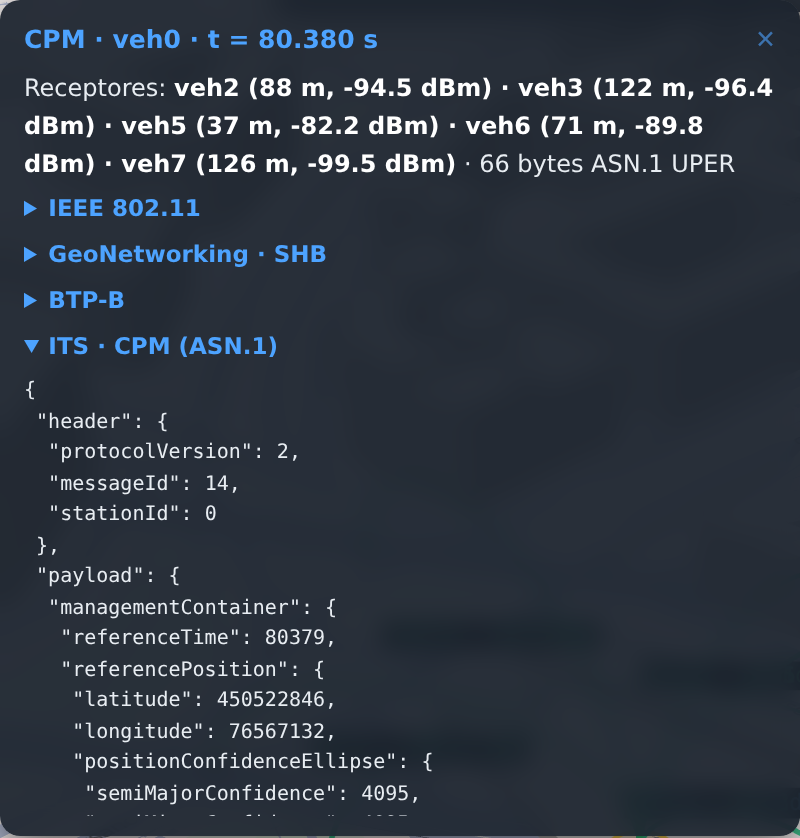
\includegraphics[width=0.55\textwidth]{img/popup_mensaje.png}
\caption{Clic sobre un pulso o arco: disección por capas plegables (802.11
$\rightarrow$ GeoNetworking $\rightarrow$ BTP-B $\rightarrow$ ITS) con el
ASN.1 completo y los receptores con distancia y RSSI.}
\label{fig:popup}
\end{figure}

% ============================================================================
\section{Parte 3 --- Los mismos pcaps con Wireshark}
% ============================================================================

\begin{enmac}
\begin{lstlisting}[language=bash]
open ~/van3twin-docker/results/v2v-EVA-0-0.pcap   # pcap del nodo 0 (ambulancia)
\end{lstlisting}
\end{enmac}

Filtros de visualización útiles (barra superior):

\begin{center}
\small
\begin{tabular}{@{}ll@{}}
\toprule
\textbf{Filtro} & \textbf{Muestra} \\
\midrule
\texttt{gnw} & Todo GeoNetworking (incluye \emph{beacons} sin payload) \\
\texttt{btpb.dstport == 2001} & Solo CAM \\
\texttt{btpb.dstport == 2009} & Solo CPM \\
\texttt{its} & Mensajes ITS decodificados (CAM/DENM\ldots) \\
\texttt{its.stationID == 0} & Solo los mensajes de la estación 0 \\
\texttt{wlan.sa == 00:00:00:00:00:01} & Tramas transmitidas por el nodo 0 \\
\bottomrule
\end{tabular}
\end{center}

Con una trama CAM seleccionada, el panel de detalle muestra la pila completa:
IEEE 802.11 $\rightarrow$ LLC $\rightarrow$ GeoNetworking (posición del
emisor, lifetime, hop limit) $\rightarrow$ BTP-B $\rightarrow$ ITS CAM con
\emph{cada campo} (stationID, generationDeltaTime, referencePosition, speed,
heading, contenedores de baja frecuencia\ldots). Dos herramientas más:

\begin{itemize}[leftmargin=1.6em, itemsep=2pt]
  \item \emph{Statistics $\rightarrow$ Flow Graph}: diagrama de secuencia del
        intercambio --- quién transmitió y cuándo, en orden.
  \item \emph{Statistics $\rightarrow$ I/O Graphs} con el filtro
        \texttt{btpb.dstport==2001}: tasa de CAMs vista por este nodo a lo
        largo del tiempo (compárala con las reglas de generación ETSI
        1--10\,Hz según dinámica).
\end{itemize}

% ============================================================================
\section{Parte 4 --- Contraste: qué aporta cada vista}
% ============================================================================

\begin{center}
\small
\begin{tabular}{@{}p{0.24\textwidth}p{0.34\textwidth}p{0.34\textwidth}@{}}
\toprule
\textbf{Criterio} & \textbf{Replay web 3D} & \textbf{Wireshark} \\
\midrule
Alcance & \textbf{Global}: fusiona los 20 pcaps --- toda la flota a la vez sobre el mapa & \textbf{Local}: un pcap $=$ la perspectiva de UN nodo \\
Dimensión espacial & Nativa: posiciones reales, alcance radio visible (arcos cerca/lejos) & Ausente (coordenadas como números en el detalle) \\
Dimensión temporal & Continua: play, seek, paso a paso & Lista de tramas; Flow Graph e I/O Graph como apoyo \\
Contenido del mensaje & Disección por \textbf{capas plegables} al clic (802.11/GN/BTP/ITS + JSON ASN.1) & Disección \textbf{campo a campo} con nombres ETSI, bytes exactos, y filtrable por cualquier campo \\
Agregados & PDR por par y totales (\texttt{/api/replay/info}) & Estadísticas por filtro, conversaciones, I/O graphs \\
Pérdidas & Implícitas: arco ausente $=$ no recibido & Explícitas comparando pcap del emisor vs.\ receptor \\
Ideal para & Entender la \emph{dinámica}: quién oye a quién, cuándo y dónde & Verificar el \emph{protocolo}: formato, campos, tiempos exactos, depuración \\
\bottomrule
\end{tabular}
\end{center}

\begin{notabox}
Regla práctica: la web responde ``\emph{¿qué pasó en la corrida?}'';
Wireshark responde ``\emph{¿qué dice exactamente esta trama?}''. En un
análisis real se usan en ese orden: localizar el evento en el replay
(instante y vehículos implicados) y abrir después el pcap correspondiente en
Wireshark filtrando por \texttt{its.stationID} y el instante.
\end{notabox}

% ============================================================================
\section{Interpretación de los datos de señal}
% ============================================================================

Con el parche SignalInfo activo, cada fila de \texttt{signal-rx.csv} es una
recepción: \texttt{rx} (estación receptora), \texttt{tx} (emisora),
\texttt{t\_ms} (instante simulado), \texttt{rssi} (potencia recibida, dBm) y
\texttt{snr} (margen señal/ruido, dB). En el visor, la etiqueta de cada
enlace muestra \emph{distancia · RSSI} de esa recepción concreta.

\textbf{La escala dBm es logarítmica}: $-45$\,dBm es una señal muy fuerte
(vecino pegado), $-80$\,dBm una débil, y cada $-10$\,dB es $10\times$ menos
potencia. La sensibilidad de 802.11p a 12\,Mbit/s ronda los $-85$/$-92$\,dBm:
un enlace por debajo empieza a perder tramas (se refleja en el PDR del par y
en el PER global).

\textbf{Modelo log-distancia.} En espacio urbano la potencia cae como
\[ \mathrm{RSSI}(d) \;=\; A \;-\; 10\,n\,\log_{10}(d), \]
donde $n$ es el \emph{exponente de propagación} (2 en espacio libre;
2,5--3,5 urbano). Ejemplo real de una corrida de esta práctica: 6\,m
$\rightarrow -45{,}8$\,dBm y 135\,m $\rightarrow -81{,}7$\,dBm; la caída de
35,9\,dB en $\log_{10}(135/6)=1{,}35$ décadas da $n \approx 2{,}7$. Regla
rápida con ese $n$: \textbf{duplicar la distancia cuesta $\sim$8\,dB}.

\textbf{Presupuesto de enlace}: con $P_{tx}=30$\,dBm, la pérdida de
propagación es $PL(d) = P_{tx} - \mathrm{RSSI}(d)$ (75,8\,dB a 6\,m;
111,7\,dB a 135\,m en el ejemplo). \textbf{SNR}: es el RSSI menos el suelo de
ruido; la tasa del EVA (16-QAM~1/2 a 12\,Mbit/s en 10\,MHz) necesita
$\mathrm{SNR}\gtrsim 11$\,dB para decodificar (tabla~\ref{tab:sens}) ---
recepciones con SNR menor deberían ser raras (el modelo de error las descarta
y ni aparecen en el CSV).

% ============================================================================
\section{Ejercicios}
% ============================================================================

\begin{tareabox}
\begin{enumerate}[leftmargin=1.6em, itemsep=3pt]
  \item Con el replay en modo paso y el filtro ``veh0'', mide cuántos
        receptores tiene un CAM de la ambulancia en el minuto 1 y en el
        minuto 2. Explica la diferencia con las posiciones del mapa.
  \item Toma un CAM concreto en la web (clic $\rightarrow$ anota
        \texttt{stationID} y $t$) y encuentra \emph{la misma trama} en
        Wireshark (filtro \texttt{its.stationID} + instante). Compara el
        contenido decodificado en ambas vistas.
  \item Del \texttt{/api/replay/info}, elige el par con PDR más bajo y el más
        alto. Verifica en el replay (posiciones) por qué, y contrasta en
        Wireshark contando tramas de ese emisor en el pcap del receptor.
  \item Con I/O Graphs, obtén la tasa de CAMs del nodo 0 en el tiempo y
        relaciónala con su velocidad (reglas de generación ETSI: más dinámica
        $\Rightarrow$ más CAMs).
  \item Del panel \textbf{PHY 802.11p}: anota el rango de cobertura p95 y el
        PER global. Con potencia TX de 30\,dBm y el modelo de propagación
        urbano, ¿es coherente ese alcance? Verifica en el replay un arco
        cercano al máximo observado.
\end{enumerate}
\end{tareabox}

\begin{tareabox}
\textbf{Interpretación de señal (requiere \texttt{signal-rx.csv})}
\begin{enumerate}[leftmargin=1.6em, itemsep=3pt, resume]
  \item \textbf{Estimar el exponente de propagación.} En modo paso, anota 5+
        etiquetas (distancia, RSSI) de enlaces del mismo emisor. Ajusta
        $\mathrm{RSSI}=A-10\,n\log_{10}(d)$ (dos puntos bastan; mejor una
        regresión) y obtén $n$. ¿Coincide con el $n\approx2{,}7$ del ejemplo?
        ¿Qué modelo de propagación configura el EVA en ns-3?
  \item \textbf{Curva RSSI--distancia.} Copia \texttt{signal-rx.csv} al Mac,
        cruza cada fila con la distancia (etiquetas del visor o el campo
        \texttt{receivers\_info} del popup) y grafica la dispersión
        RSSI vs.\ $\log_{10}(d)$ (Excel o Python). Superpón tu ajuste del
        ejercicio anterior. ¿Hay valores muy alejados de la recta? ¿A qué los
        atribuyes (edificios, interferencia entre transmisiones simultáneas)?
  \item \textbf{Sensibilidad y alcance máximo.} Busca en el CSV el RSSI
        mínimo con el que hubo recepción correcta. Compáralo con la
        sensibilidad nominal de 802.11p a 12\,Mbit/s ($\sim -85$\,dBm) y
        despeja de tu modelo la distancia máxima teórica
        $d_{max}$. Contrasta con el ``rango máximo observado'' del panel PHY.
  \item \textbf{SNR y decodificación.} Haz el histograma de la columna
        \texttt{snr}. ¿Cuál es el mínimo observado? Relaciónalo con el umbral
        de 16-QAM~1/2 (tabla~\ref{tab:sens}) y explica por qué no aparecen
        recepciones por debajo.
  \item \textbf{Presupuesto de enlace.} Para tres etiquetas del visor a
        distintas distancias, calcula $PL(d)=30\,\mathrm{dBm}-\mathrm{RSSI}$
        y verifica que crece $\sim 10\,n$ dB por década de distancia.
\end{enumerate}
\end{tareabox}

\vspace{6pt}\hrule\vspace{6pt}

{\small\emph{Documentos relacionados:}
\texttt{Manual\_Simulacion\_VaN3Twin\_SUMO\_GEO.pdf} (operación del stack y
del replay), \texttt{GUIA\_INTEGRACION\_SUMO\_GEO.md},
\texttt{CONTEXTO\_SUMO\_GEO.md} (arquitectura técnica del replay).}

\end{document}
